\chapter{FUNDAMENTAÇÃO TEÓRICA}\label{ch:fundaments-teorico}
A mineração de dados é um assunto totalmente interdisciplinar, podendo ser definido de diversas maneiras. Até mesmo o termo \textit{data mining} não representa realmente todos os componentes desta área. \citeonline{han} exemplificam esta questão comentando sobre a mineração de ouro através da extração de rocha e areia, que é chamado de mineração de ouro e não mineração de rochas ou mineração de areia. Analogamente, a mineração de dados deveria se chamar "mineração de conhecimento através de dados" que, infelizmente, é um termo um tanto longo. Entretanto, uma referência mais curta, como "mineração de conhecimento", pode não enfatizar a mineração de uma enorme quantidade de dados. Apesar disso, a mineração é um termo que caracteriza o processo de encontrar uma pequena quantia de uma preciosa pepita em uma grande quantidade de matéria bruta. Nesse sentido, um termo impróprio contendo ambos \textit{"data"} e \textit{"mining"} se tornou popular e, como consequência, muitos outros nomes similares surgiram: \textit{knowledge mining from data}, \textit{knowledge extraction}, \textit{data/pattern analysis}, \textit{data archaeology} e \textit{data dredging}.

Na seção~\ref{sec:kdd} será abordado os conceitos de descoberta de conhecimento em base de dados e a sua diferença em relação ao \textit{data mining}. Logo após a explicação desta distinção, será apresentado os métodos e a concepção de \textit{data mining}. Alguns desses métodos tem como prática o uso de aprendizado de máquina, que será definido na seção~\ref{sec:machine-learning}. A seção~\ref{sec:python} irá caracterizar a linguagem de programação Python e qual a sua vantagem em utilizá-la para a mineração de dados.

%%
% KDD
\section{DESCOBERTA DE CONHECIMENTO EM BASE DE DADOS E \textit{DATA MINING}}\label{sec:kdd}
Muitas pessoas tratam a mineração de dados como um sinônimo para outro termo muito popular, descoberta de conhecimento em base de dados (\textit{knowledge discovery from data}) - KDD, enquanto outros referenciam \textit{data mining} como apenas uma etapa no processo de descoberta de conhecimento em base de dados. O processo de KDD é demonstrado através da  Figura~\ref{kdd-fig} e, posteriormente, listada como uma sequência interativa e iterativa dos seguintes passos: \\ \\ \\ \\ \\ \\

\begin{figure}
	\centering
	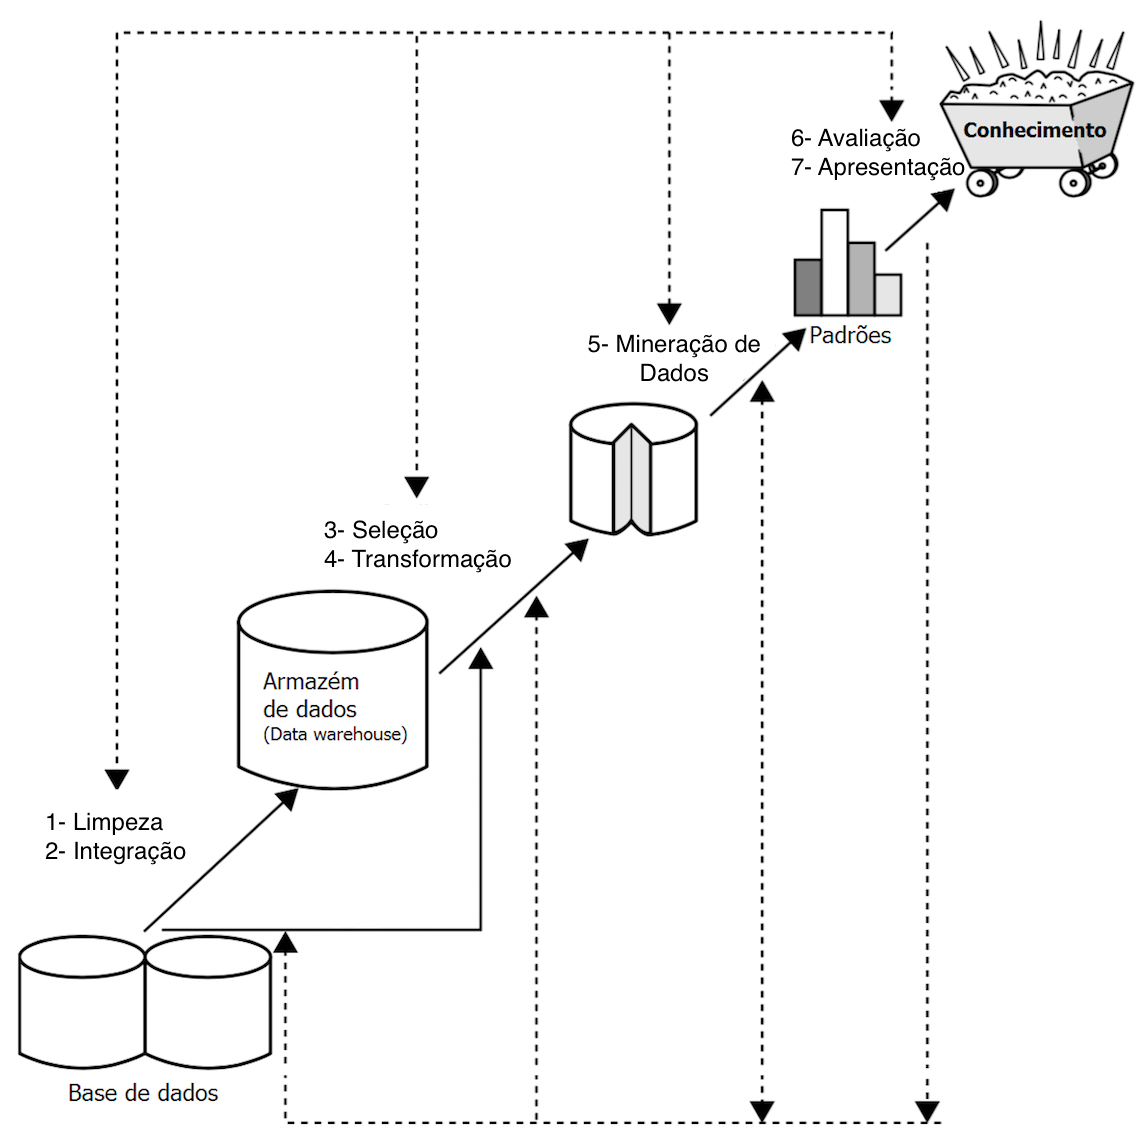
\includegraphics[width=1\textwidth]{Cap3/imagens/kdd2}
	\caption{Etapas do processo de KDD}
	\vspace{-0.3cm}
	\legend{FONTE: Adaptado de \citeonline{han}}
	\label{kdd-fig}
\end{figure}

\begin{enumerate}
	\item \textit{Data cleaning} (Limpeza de dados);
	\item \textit{Data integration} (Integração de dados);
	\item \textit{Data selection} (Seleção de dados);
	\item \textit{Data transformation} (Transformação de dados);
	\item \textit{Data mining} (Mineração de dados);
	\item \textit{Pattern evaluation} (Avaliação de padrões);
	\item \textit{Knowledge presentation} (Apresentação de conhecimento).
\end{enumerate}

É importante notar que algum dos processos acontecem na mesma etapa: Limpeza e integração; Seleção e transformação; Avaliação e apresentação.

De acordo com \apudonline{brachman}{fayyad2}, as etapas são interativas porque envolvem a cooperação da pessoa responsável pela análise de dados, cujo conhecimento sobre o domínio orientará a execução do processo. Por sua vez, a interação deve-se ao fato de que, com frequência, esse processo não é executado de forma sequencial, mas envolve repetidas seleções de parâmetros e conjuntos de dados, aplicações das técnicas de \textit{data mining} e posterior análise dos resultados obtidos, a fim de refinar os conhecimentos extraídos.

KDD refere-se ao processo global de descobrimento de conhecimento útil em bases de dados. \textit{Data mining} é um passo particular neste processo de aplicação de algoritmos específicos para extrair padrões (modelos) de dados. Os passos adicionais no processo KDD, como integração de dados, limpeza, seleção e transformação dos dados, assim como a interpretação e a apresentação dos resultados, asseguram que o conhecimento útil (informação) foi descoberto provenientes da etapa de mineração \cite{han}. A aplicação cega de métodos de \textit{data mining}, conforme alertado por \citeonline{navega}, pode ser uma atividade perigosa que conduz a descoberta de padrões sem sentido. 

O KDD evoluiu e continua evoluindo da interseção de pesquisas em campos como bancos de dados, aprendizado de máquinas (\textit{machine learning}), reconhecimento de padrões, estatísticas, inteligência artificial, aquisição de conhecimento para sistemas especialistas, visualização de dados, descoberta científica, recuperação de informação e computação de alto-desempenho. Aplicações de KDD incorporam teorias, algoritmos e métodos de todos estes campos \cite{credito-bancario}.


%%
%% Data Mining
%\section{\textit{DATA MINING}}\label{sec:data-mining}
Apesar do conceito de \textit{data mining}, na maioria das vezes, ser utilizado pelas indústrias, mídias e centros de pesquisa para se referir ao processo de descoberta de conhecimento considerado em sua globalidade, o termo \textit{data mining} pode ser usado também para indicar o quinto estágio do KDD, sendo um processo essencial na descoberta e extração de padrões de dados. \citeonline{han}, adotam uma visão mais abrangente para a funcionalidade de mineração de dados: \textit{data mining} é o processo de descoberta de padrões interessantes e conhecimentos de um vasto conjunto de dados. A fonte dos dados pode ser banco de dados, \textit{data warehouses}, a Internet, outros repositórios de informações, ou dados correntes em sistemas dinâmicos.

Uma das definições, talvez, mais importante de \textit{data mining} foi elaborada por \citeonline{fayyad} "...o processo não-trivial de identificar, em dados, padrões válidos, novos, potencialmente úteis e ultimamente compreensíveis".

\textbf{\textcolor{red}{[MELHORAR]}} \textit{Data mining} ou mineração de dados, pode ser entendido então, como o processo de extração de informações, sem conhecimento prévio, de algum conjunto de dados e seu uso para tomada de decisões. A mineração de dados se define através de processos automatizados de captura e análise deste conjunto de dados com a finalidade de extrair algum significado, podendo descrever características do passado, como também para predizer futuras tendências \cite{conceito-data-mining}.

Diversos métodos são usados em \textit{data mining} para encontrar respostas ou extrair conhecimento interessante. Esses podem ser obtidos através dos seguintes métodos:

\begin{itemize}
	\item Classificação: associa ou classifica um item a uma ou várias classes. Os objetivos dessa técnica envolvem a descrição gráfica ou algébrica das características diferenciais das observações de várias populações. A ideia principal é derivar uma regra que possa ser usada para classificar, de forma otimizada, uma nova observação a uma classe já rotulada;
	
	\item Modelos de Relacionamento entre Variáveis: associa um item a uma ou mais variáveis de predição de valores reais, conhecidas como variáveis independentes ou exploratórias. Nesta etapa se destacam algumas técnicas estatísticas como regressão linear simples, múltipla e modelos lineares por transformações, com o objetivo de verificar o relacionamento funcional entre duas variáveis quantitativas, ou seja, constatar se há uma relação funcional entre X e Y;
	
	\item Análise de Agrupamento (\textit{Cluster}): associa um item a uma ou várias classes (ou \textit{clusters}). Os \textit{clusters} são definidos por meio do agrupamento de dados baseados em modelos probabilísticos ou medidas de similaridade. Analisar \textit{clusters} é uma técnica com o objetivo de detectar a existência de diferentes grupos dentro de um determinado conjunto de dados e, caso exista, determinar quais são eles;
	
	\item Sumarização: determina uma descrição compacta para um determinado subconjunto, por exemplos; medidas de posição e variabilidade. Nesta etapa se aplica algumas funções mais sofisticadas envolvendo técnicas de visualização e a determinação de relações funcionais entre variáveis. Estas funções são usadas para a geração automatizada de relatórios, sendo responsáveis pela descrição compacta de um conjunto de dados;
	
	\item Modelo de Dependência: descreve dependências significativas entre variáveis. Estes modelos existem em dois níveis: estruturado e quantitativo. O nível estruturado demonstra, através de gráficos, quais variáveis são localmente dependentes. O nível quantitativo especifica o grau de dependência utilizando alguma escala numérica;
	
	\item Regras de Associação: determinam relações entre campos de um banco de dados. Esta relação é a derivação de correlações multivariadas que permitam auxiliar as tomadas de decisão. Medidas estatísticas, como correlação e testes de hipóteses apropriados, revelam a frequência de uma regra no universo dos dados minerados;
	
	\item Análise de Séries Temporais: determina características sequênciais, como dados com dependência no tempo. Tem como objetivo modelar o estado do processo extraindo e registrando desvios e tendências no tempo. As séries são compostas por quatro padrões: tendência, variações cíclicas, variações sazonais e variações irregulares. Existem vários modelos estatísticos que podem ser aplicados a essas situações.
\end{itemize}

A maioria destes métodos são baseados em técnicas de aprendizado de máquina (\textit{machine learning}), reconhecimento de padrões e estatística. Essas técnicas vão desde estatística multivariada, como análise de agrupamentos e regressões, até modelos mais atuais de aprendizagem, como redes neurais, lógica difusa e algoritmos genéticos \cite{conceito-data-mining}.

Devido aos vários métodos estatísticos que são aplicados no processo de \textit{data mining}, \citeonline{fayyad} mostram uma relevância da estatística para o processo de extração de conhecimentos ao afirmar que essa ciência provê uma linguagem e uma estrutura para quantificar a incerteza resultante quando se tenta deduzir padrões de uma amostra a partir de uma população.

%%
% Machine Learning
\section{\textit{MACHINE LEARNING}}\label{sec:machine-learning}
Abstratamente, pode-se pensar em \textit{machine learning}, ou aprendizado de máquina, como um conjunto de ferramentas e métodos que tentam inferir padrões e extrair \textit{insights} de uma porção daquilo que se é observado no mundo. Por exemplo, ao tentar ensinar um computador a reconhecer os códigos postais escritos nos envelopes, os dados podem consistir em fotografias dos envelopes, além de um registro do código postal a que cada envelope estava endereçado, ou seja, dentro de um contexto, é possível selecionar um registro de ações de certos objetos, aprender com este registro e, em seguida, criar um modelo dessas atividades que irão informar a compreensão deste contexto futuramente \cite{machine-hacker}.

Na prática, isto requer dados e, em aplicações atuais, isso, muitas vezes, significa uma grande quantidade de dados (talvez vários \textit{terabytes}). A maioria das técnicas de aprendizagem automática considera a disponibilidade de tais dados como algo inquestionável, o que significa novas oportunidades para a sua aplicação, em função da quantidade de dados que são produzidos como um produto de administrar companhias modernas.

\textit{Machine learning} é a intersecção entre ciência da computação, engenharia, estatística e outras disciplinas. É possível ser aplicada em várias áreas, desde políticas a geociência. É uma ferramenta que pode ser utilizada para a solução de vários problemas. Qualquer campo que precisa interpretar e agir sobre dados pode se beneficiar do uso de técnicas de \textit{machine learning} \cite{machine-hacker}.

A prática de engenharia está em utilizar a ciência para resolver um problema. Em engenharia, é comum resolver um problema determinista, em que a solução dada por humanos sempre resolve o problema. Se desenvolver um software para controlar uma máquina de venda automática é melhor que esta trabalhe sempre, independentemente do dinheiro depositado ou dos botões pressionados. Muitos problemas existem quando a solução não é determinista, isto é, ou não se sabe o suficiente sobre o problema ou não se tem poder computacional suficiente para delineá-lo adequadamente. Para esses problemas, precisa-se de estatísticas. 

Uma das tarefas de \textit{machine learning} é a classificação. Na classificação, o trabalho é prever em que classe deve uma porção de dados ser enquadrada. Outra tarefa é a regressão que é a previsão de um valor numérico. Classificação e regressão são exemplos de aprendizado supervisionado, que são conhecidos como supervisionado, por dizer o que o algoritmo deve prever \cite{machine-learning}.

O oposto de aprendizagem supervisionada é um conjunto de tarefas conhecidas como aprendizado não supervisionado, onde não há nenhum rótulo ou valor alvo dado para os dados. \textbf{\textcolor{red}{[CONTEXTO?][}}A tarefa através da qual se agrupa itens semelhantes é conhecida como \textit{clustering}.\textbf{\textcolor{red}{]}} Na aprendizagem não supervisionada, também pode-se querer encontrar valores estatísticos que descrevem os dados. Isso é conhecido como estimativa da densidade. Outra tarefa do aprendizado não supervisionado está em reduzir dados com várias funcionalidades até se chegar a um número reduzido, em que seja possível visualizá-lo em duas ou três dimensões \cite{machine-learning}.

%%
% Python
\section{LINGUAGEM PYTHON}\label{sec:python}
Python é uma linguagem de programação orientada a objetos, interpretada e interativa. Incorpora módulos, excessões e de tipagem dinâmica alta. Possui uma sintaxe clara e simples, o que facilita o aprendizado para novos desenvolvedores, assim como a rápida leitura e interpretação para usuários mais experientes. Dispõe de interfaces para várias chamadas de sistemas (\textit{system calls}) e bibliotecas, também para vários sistemas de janelas, e é extensível a outras linguagens de programação como C ou C++. É também usada como uma linguagem de extensão para aplicações que precisam de uma interface programática \cite{python-doc}.

Outra característica da linguagem Python é a portabilidade, podendo ser utilizada em diversos sistemas operacionais como variantes do Unix, em sistemas Mac e também em PCs sob MS-DOS, Windows, Windows-NT, e OS/2.

É uma linguagem de programação de alto-nível que pode ser aplicada em soluções para diversas classes diferentes. Possui uma vasta quantidade de bibliotecas que atende a áreas como o processamento de \textit{strings} (expressões regulares, Unicode, cálculo de diferença entre arquivos), protocolos de Internet (HTTP, FTP, SMTP, XML-RPC, POP, IMAP, CGI \textit{programming}), engenharia de software (testes unitários, registro de logs, \textit{profiling}, análise de código Python), e interfaces para sistemas operacionais (\textit{system calls}, sistemas de arquivos, TCP/IP \textit{sockets}) \cite{python-doc}.

A sintaxe bastante expressiva e a abundância de suas bibliotecas tornam Python uma ótima linguagem para se obter resultados em várias questões. Algumas de suas utilidades são apresentadas conforme a seguinte lista:

\begin{itemize}
	\item Escrita de \textit{scripts}: Python é uma ótima linguagem para a criação de \textit{scripts}. É possível usar \textit{scripts} para analisar arquivos de texto, gerar amostra de entradas para testar programas, coletar conteúdos de páginas \textit{web} utilizando a biblioteca \textit{Beautiful Soup}, dentre outras atividades;
	\item Desenvolvimento \textit{backend} para aplicações \textit{web}: É possível criar APIs (\textit{Application Programming Interface}, apresentado no capítulo~\ref{ch:materiais-metodos}) e interagir com banco de dados. \textit{Frameworks} mais utilizados inclui \textit{Django}, \textit{Flask} e \textit{Pyramid};
	\item Análise e visualização de dados: Conforme o foco deste trabalho, bibliotecas como \textit{pandas}, \textit{NumPy} e recursos semelhantes a outras ferramentas como R e MATLAB estão dispostas através da biblioteca \textit{SciPy};
	\item \textit{matplotlib} e \textit{Seaborn}: são mecanismos que possibilitam a visualização dos dados.
\end{itemize}

A utilização dessa linguagem como ferramenta principal para este trabalho se justifica na utilização dos pacotes que facilitam a análise e interpretação de dados. Como exemplo, \textit{NumPy}, \textit{SciPy}, \textit{pandas}, \textit{matplotlib} e \textit{IPython} são os mecanismos indispensáveis para a mineração de informações juntamente com as estruturas de dados já presentes em Python como os \textit{dictionaries} (estruturas similares ao JSON), que permitem ordenar dados através de um modelo chave-valor. Devido então a sintaxe intuitiva que a linguagem possui e seu excelente ecossistema de bibliotecas, é possível acessar APIs e manipular dados com mais facilidade \cite{mining-social-web}.













